\chapter{Evaluation des Prototyps sowie der Wirkung des Prototyps auf das Kommunikationsverhalten der Probanden}

Dieser Abschnitt behandelt das Testen der umgesetzten Anwendung sowie das Messen des Effektes, den die Anwendung haben soll. Er zeigt auf, an welchen Elementen des Prototyps Weiterentwicklungen von Nöten sind und gibt erste Ergebnisse darauf, wie seine Wirkung ist.

% Die beiden Studienschwerpunkte 


\section{Methodik}
% Die Evaluationsphase zielt primär darauf ab in der Kommunikationsforschung von asymmetrischen-Multiplayer Spielen neue Erkenntnisse zu liefern. Der gewählte Ablauf der primären Forschungsstudie erfolgt innerhalb eines kleines Experimentes, bei dem die Probanden zunächst nicht den Zweck der Studie erfahren. DIe Ergebnisse dieses Experiments werden auf quantitative Weise erfasst.
% % Die gewählte Methodik der Bewertung des Einflusses auf die Probanden ist dabei diejenige, die bei den zugrunde Legenden Arbeiten für ihre quantitativen Ergebnisse verwendet wurde. 

% Während der Kommunikationseinfluss im Vordergrund steht, wird ebenfalls auch die entwickelte Anwendung geprüft. Bei der hierfür gewählten Forschungsmethode wurden quantitative als auch qualitative Daten gesammelt. Diese dienen dazu einen Kenntnis stand darüber zu erhalten, an welchen Aspekten die Anwendung weiterentwickelt werden muss.
% Die Evaluation der Anwendung erfolgt über standardisierte Fragebögen, die in vergleichbaren Studien ebenfalls auf diese Weise verwendet wurden. Zusätzlich wurden über einen anderen Fragebogen qualitative Ergebnisse eingeholt.

Dieser Abschnitt beschreibt die methodische Herangehensweise zur Evaluation der entwickelten Anwendung im Kontext der Kommunikationsforschung bei asymmetrischen-Multiplayer Spielen. Ziel war es, sowohl die kommunikative Wirkung der Anwendung als auch ihre funktionale und gestalterische Tauglichkeit zu Untersuchung. Die gewählte Vorgehensweise kombiniert qualitative und quantitative Methoden innerhalb eines experimentellen Studiensettings, um ein möglichst umfassendes Bild der Nutzung und der Interaktionen zu gewinnen.

\subsection{Forschungsdesign}
Zur Untersuchung der Forschungsfragen \say{Welche Verbesserungen in der Kommunikation zwischen den Anwendern können durch ein asymmetrisches Multiplayer-Spiel mit zwei verschiedenen Spielerklassen beobachtet werden?} und \say{Wie stehen die Nutzer zu einem spielerischen Ansatz und zur Verbesserung der Kommunikation, insbesondere auch im Umgang mit Fremden?} wurde ein praxisorientiertes, experimentelles Forschungsdesign gewählt. Im Zentrum steht das asymmetrische-Multiplayer-Szenario, in dem jeweils zwei Personen unterschiedliche Rollen mit ungleich verteilten Informationen übernehmen. Diese Konstellation ermöglicht es, die Wirkung der Anwendung auf kooperative Kommunikationsprozesse zu analysieren.

Das Design sieht in der Erhebung sowohl quantitative als auch qualitative vor. 

\subsection{Erhebungsinstrumente}
Die Datenerhebung dieser Studie erfolgte mittels standardisierte Fragebögen zu den Themen System Usability, Immersion, Spiel Erfahrung Motivation und dem Workload. Außerdem wurden über standardisierte Fragebögen die Entwicklung des affektiven Status, der Beziehung zueinander und Leadership. Außerdem wurden neu erstelle Fragebögen zum Thema Umgang mit fremden Menschen und Demographie verwendet.

Zusätzlich wurden Videoaufnahmen von der Versuchsdurchführung gemacht, die zur Auswertung der Kommunikationsentwicklung notwendig sind.

\subsection{Stichprobe}
[hier quellen finden zu stichproberngröße bei statistischen auswertungen, expiermenten bei denen 2 oder mehrere personen mitmachen und zu qualitativer forschung]

\subsection{Durchführung der Studie}
Zunächst wurden Probanden über Einladungsnachrichten in diversen Chatgruppen, sowie mehrere Rundmails gesucht und eingeladen. Sie konnten sich in einer Terminkalender-Anwendung in einen für den Probandentest verfügbaren Zeitslot eintragen.

Beim Probandentest wurden die Teilnehmer zunächst begrüßt und mussten eine Einverständniserklärung unterzeichnen, da sie während des Versuchsdurchlaufes gefilmt wurden. Den Probanden wurde zunächst nicht erklärt um was es in dem Versuchsdurchlauf im Detail geht. Sie wussten zunächst nur, dass sie einen asymmetrischen Multiplayer spielen dürfen, bei denen zu zweit Rätsel gelöst werden müssen und jeder Spielteilnehmer eine andere Rolle im Spiel einnehmen wird. Das gezielte Verschweigen des Sinns der Nutzerstudie wurde gemacht, damit die Teilnehmer nicht voreingenommen in die Aufgaben des Versuchsaufbaus gehen. Dies würde sonst dazu führen, dass die Ergebnisse verfälscht werden. Die Art der Anleitung orientierte sich dabei an die des Milgram Experiments 1963 (vgl. \cite{milgram_behavioral_1963}) bei dem den Probanden ebenfalls nicht der eigentliche Zweck des Versuches erklärt wurde, damit das Ergebnis nicht verfälscht wird. Sie haben lediglich Anweisungen zu den Aufgaben, die sie machen mussten erhalten. 

Zu Beginn des Versuchsdurchlaufs füllten die Probanden den demografischen Fragebogen aus, bei dem Alter, Geschlecht und Vorerfahrungen mit Spielen, Multiplayer-Spielen und Touchsteuerungen aus. Anschließend folgten die standardisierten Fragebögen zur gegenseitigen Beziehung, zum Spielertyp und den aktuellen affektiven Status aus.

Der Kern der Versuchsdurchführung wird in 3 Komponenten geteilt. Die Hauptkomponente ist das Spielen des Prototyps, welcher zwischen einem Vortest und Nachtest gespielt wurde.

Die Probanden mussten nun zunächst den Vortest absolvieren. 

\begin{figure}[ht]
\centering
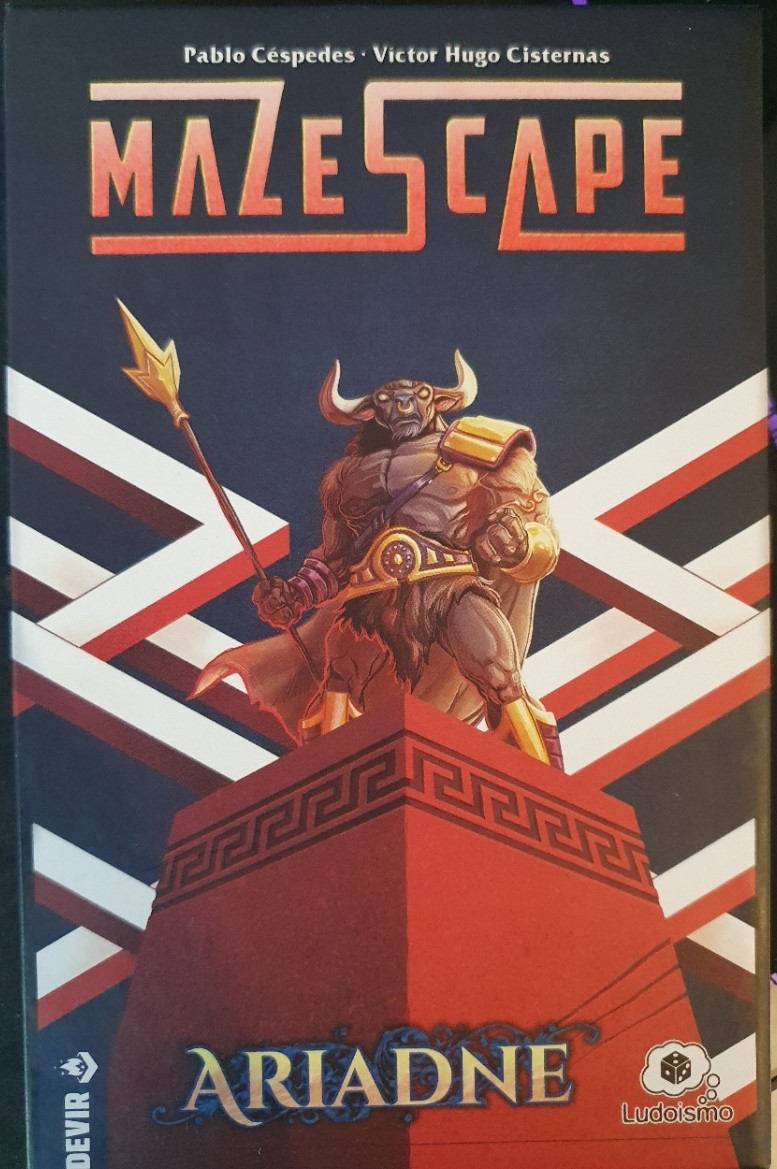
\includegraphics[width=1\linewidth]{content/pictures/MazeScape.jpg}
\caption{Verpackung des Spiels MazeScape (vgl. \cite{noauthor_mazescape_nodate})}
\label{fig:mazescape}
\end{figure}

\begin{figure}[ht]
\centering
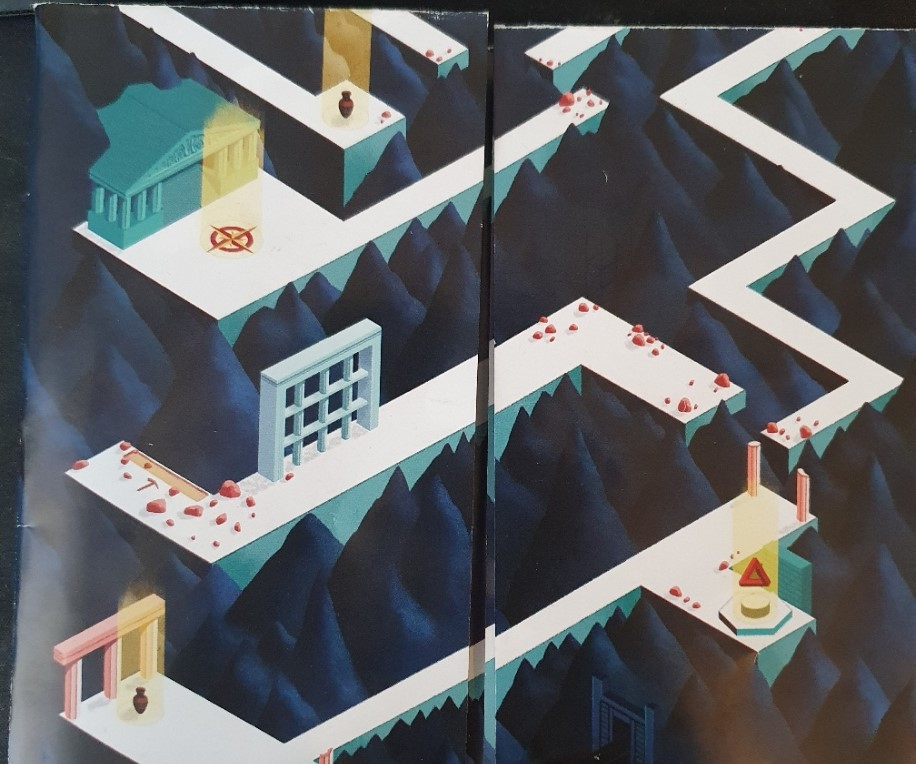
\includegraphics[width=1\linewidth]{content/pictures/MazeScape_Level02.jpg}
\caption{Level 02 aus dem Spiel MazeScape (vgl. \cite{noauthor_mazescape_nodate})}
\label{fig:mazescape_level-02}
\end{figure}

% Der Vortest umfasste das Spielen eines Levels aus dem Spiel MazeScape (vgl. Abbildung \ref{fig:mazescape}). Die Regeln wurden für den Anwendungszweck abgeändert. Die Probanden mussten zu zweit die 
Der Vortest umfasste das Spielen des zweiten Levels (vgl. Abbildung \ref{fig:mazescape_level-02}) aus dem Spiel \say{MazeScape} (vgl. Abbildung \ref{fig:mazescape}). Die grundlegenden Regeln des Spiels bezüglich der Bewegung durch die Spielwelt wurden für diesen Anwendungszweck übernommen. Die weiteren Regeln den Spiels zu bestimmten Gegenständen, Punkten oder Gegnern wurden aus dem Grund der fehlenden Relevanz nicht berücksichtigt. Die Probanden hatten zehn Minuten Zeit um gemeinsam vom Startpunkt im Level an das Ziel zu kommen. Es war dabei nicht wichtig rechtzeitig ans Ziel zu kommen.

Dieser Vortest wurde gemacht, damit ein Grundwert der bestehenden Kommunikation zwischen den Probanden zu bestimmen. Dieser sollte sich nach dem Nachtest verbessert haben.

Nach erfolgreich oder nicht erfolgreichem Abschluss des Vortests durften die Probanden den Prototyp von Connecting-Minds testen. Sie erhielten zunächst eine Einführung zur Steuerung der jeweiligen Anwendung. Anschließend durften sie starten. Sie hatten hierfür 40 Minuten Zeit. Ziel war es, die Rätsel zu lösen, allerdings war es nicht wichtig, ob sie das Tutorial erfolgreich in der gegebenen Zeit abschließen.

Die Zuordnung welcher Proband welche Spielrolle einnimmt, wurde nach der Begrüßung der Probanden vollzogen. Für die ersten Fragebögen war es wichtig zu wissen, wer welche Rolle im Spiel einnimmt. Daher erfolgt zum Ausfüllen der Einverständniserklärung die Einteilung von den Probanden ausgehend.

Nach absolvieren des Prototyps mussten die Probanden die Fragebögen zu den Themen System Usability, Immersion, Spiel Erfahrung Motivation und dem Workload des jeweiligen Probanden ausfüllen.

Im Anschluss folgte nun der Nachtest. Hierfür mussten die Probanden erneut ein Level aus dem Spiel MazeScape spielen. Sie spielten dabei das Level 3 (vgl. Abbildung \ref{fig:mazescape_level-03}). Wie im Vortest wurden die gleichen Regeln zur Bewegung durch die Spielwelt für den Versuch angewandt. Alle anderen Regeln wurden ebenfalls nicht berücksichtigt. Die Schwierigkeit, die sich in diesem Level für die Probanden ergeben hat, ist dass sie dass Ziel zunächst zusammen suchen müssen ehe sie einen Weg durch das Labyrinth finden können.

\begin{figure}[ht]
\centering

\includegraphics[width=1\linewidth]{content/pictures/MazeScape_Level03.jpg}
\caption{Level 03 aus dem Spiel MazeScape (vgl. \cite{noauthor_mazescape_nodate})}
\label{fig:mazescape_level-02}
\end{figure}

Wie im Vortest hatten die Probanden hierfür ebenfalls zehn Minuten Zeit. Außerdem war es ebenso nicht wichtig das Ziel zu erreichen.

Nach Abschluss wurden die letzten Fragebögen von den Probanden ausgefüllt. Sie behandelten Vergleichswerte im Bezug auf die gegenseitige Beziehung und dem affektiven Status. Außerdem mussten sie Fragebögen zum Thema Leadership und dem Umgang mit Menschen in diesem Versuchsaufbau ausfüllen. Zuletzt hatten sie noch ein Freitextfeld, bei dem ihr qualitatives Feedback zur Anwendung gegeben werden konnte.

Nachdem alle Fragebögen ausgefüllt wurden, wurde die Aufnahme beendet und es wurde sich bei den Probanden für die Teilnahme bedankt. Sie durften sich noch etwas von den bereitgestellten Snacks nehmen und wurden im Anschluss entlassen.

Die gesamte Versuchsdurchführung dauerte etwa 75 Minuten pro Probanden-paar.

\subsection{Rahmenbedingungen}


\section{Ergebnisse}

% \section{Zielsetzung}

% \section{Planung und Durchführung}

% \section{Auswertung der Tests}

